\section{Logs}\label{sec:logs-storing}

El següent conjunt de paràmetres és el que permet agrupar tota la informació present als \textit{\gls{log}s}.
L’evolució al llarg dels anys no ha afectat gaire respecte als paràmetres existents sinó al contingut d’aquests. \\

\noindent
Aquí un exemple d’un \textit{log}:

\begin{itemize}
    \item \texttt{ip\_address:  39.92.248.6}
    \item \texttt{date: 20/Apr/2011}
    \item \texttt{time: 23:59:59 +0200}
    \item \texttt{request}:
    \begin{itemize}
        \item \texttt{method: GET}
        \item \texttt{resource: /e-prints/bitstream/2117/8469/1/sdarticle.pdf}
        \item \texttt{version: HTTP/1.0}
        \item \texttt{status\_code: 304}
        \item \texttt{response\_size: -}
    \end{itemize}
    \item \texttt{referer: null}
    \item \texttt{user\_agent:  gsa-crawler (Enterprise; T2-QGG2U8NZXNSAA upcnet\\.backoffice.aps@upcnet.es)}
\end{itemize}


\noindent \\
Aquesta estructura de dades representa la informació que podem extreure directament dels \textit{\gls{log}s} provinents d'\gls{UPCommons}.
El resultat del nostre processament d'aquests altera aquest format per afegir més informació, com veurem més endavant.

\clearpage

\subsection{Bases de dades candidates}\label{subsec:log-db-options}

\noindent \\
A continuació llistarem les opcions candidates a ser el sistema gestor de bases de dades on emmagatzemarem tots els logs.

\noindent \\
La majoria són sistemes d’agregació de logs, que incorporen eines de monitoratge, sistemes d’alertes, visualització, etc.
És criteri nostre fer-ne ús d’aquests serveis o només continuar amb la base de dades.

\noindent \\
Com a primeres opcions considerem aquelles que siguin de programari lliure i en les quals puguem instal·lar localment la base de dades.

\noindent \\
\textbf{Grafana Loki~\cite{loki:main}}\label{subsubsec:log-db-option-loki}

\noindent \\
\textit{Grafana Labs} proporciona \textit{Loki}, un sistema d’agregació de \textit{\gls{log}s} de codi obert, basat en Prometheus.
És un sistema distribuït i dissenyat per ser escalable.
Les seves característiques principals són:

\begin{itemize}
    \item \textbf{Escalabilitat}: Disposa de diferents modes de desplegament on pots escollir el que més s’adapti als teus requisits.
    \item \textbf{Integració}: Suporta diverses implementacions/llibreries de tercers per fer-ne servir, i diversos modes de desplegament en local.
    \item \textbf{Grafana}: Integració per defecte amb \textit{Grafana} com a eina principal d’observabilitat.
    \item \textbf{Emmagatzemament}: Loki només indexa les metadades dels \textit{\gls{log}s}~\cite{loki:indexing}, és a dir, només el \textit{\gls{timestamp}} i els \textit{labels} definits.
    El contingut del \textit{\gls{log}} no s’indexa.
    Utilitzant aquest plantejament, s’aconsegueix reduir la quantitat total d'espai de disc necessari.
    \begin{itemize}
        \item Aquesta característica és bastant interessant si utilitzem aquests \textit{labels} per afegir informació relacionada amb el recurs accedit per a després com a millorar el procés de cerca.
    \end{itemize}
\end{itemize}

\clearpage

\noindent
\textbf{Elastic~\cite{elastic}}

\noindent \\
Elastic, conegut pel seu motor de cerca Elasticsearch, disposa d’una solució de monitoratge de \textit{\gls{log}s}.
Les seves característiques principals:

\begin{itemize}
    \item \textbf{Escalabilitat}: dissenyat per monitorar \textit{\gls{log}s} fins a una escala de \textit{petabytes}.
    \item \textbf{Integració}: suporta diverses implementacions/llibreries de tercers per fer-ne servir, i modes de desplegament en local.
    \item \textbf{\textit{Logstash}}: mecanisme per centralitzar i transformar les dades per a després emmagatzemar-les a qualsevol lloc.
    \item \textbf{\textit{Kibana}}: integració per defecte amb \textit{Elastic Kibana} com a eina principal d’observabilitat.
    \item \textbf{Categorització}: incorpora una eina per identificar patrons, tendències i anomalies als \textit{\gls{log}s}.
\end{itemize}


\noindent \\
\textbf{Apache SOLR~\cite{SOLR}}

\noindent \\
Apache SOLR és una plataforma de cerca que es pot utilitzar com a mecanisme d’emmagatzemament de documents. 
Les seves característiques principals:

\begin{itemize}
    \item \textbf{Escalabilitat}: basat en un sistema distribuït i rèpliques, és optimitzat per grans volums de dades.
    \item \textbf{Integració}: la comunicació amb el servei es realitza mitjançant l’\gls{API} de SOLR sobre \gls{HTTP} .
    També suporta diferents modes de desplegament en local.
    \item \textbf{Lucene}: fa servir \textit{Apache Lucene} com a motor de cerca principal.
\end{itemize}

\noindent
Com a contrapartida:

\begin{itemize}
    \item \textbf{Visualització}: no disposa d’un sistema de visualització de dades per defecte, així perque caldria emprar-ne un de tercers.
\end{itemize}


\clearpage

\noindent
Altres opcions que no són de codi obert són les següents,  la versió gratuïta que proporcionen és bastant limitada o no hi ha prou documentació a la xarxa són les següents:

\begin{itemize}
    \item \textbf{Graylog}~\cite{graylog}
    \item \textbf{Papertrail}~\cite{papertrail}
    \item \textbf{Loggly}~\cite{loggly}
    \item \textbf{Splunk}~\cite{splunk}
\end{itemize}

\noindent \\
\subsection{Decisió}\label{subsec:log-db-decision}

\noindent
La primera decisió presa fou donar suport a \textit{Grafana Loki}, amb els motius que llistarem a continuació:

\begin{itemize}
    \item Base de dades de codi obert compatible per diferents plataformes.
    \item És una eina ben documentada~\cite{loki:documentation}.
    \item Té una gran quantitat d’usuaris actius.
    El repositori de codi~\cite{loki:code} és mantingut activament i de forma actual.
    \item Integració per defecte amb \textit{Grafana} per poder visualitzar els \textit{logs}.
    \item Diverses llibreries~\cite{loki:libraries} ja implementades per enviar \textit{\gls{log}s} a la base de dades.
    \item Com prèviament s’ha mencionat, la indexació és a partir del \textit{\gls{timestamp}} més les metadades.
    Aquestes darreres poden ser utilitzades per afegir valors que després agilitzaran el processament. \\ \\
    Com podem veure a la imatge~\ref{fig:loki-indexing}, converteixen un \textit{\gls{log}} semblant als nostres en un altre adaptat al format de loki, on utilitzen com etiqueta el tipus petició (\textit{action}) o el codi d’estat (\textit{status\_code}) \\ \\
    El nostre cas, en podem afegir uns que indiquin el tipus de \textit{\gls{log}} (cerca, accés a recurs) o marcar-ne alguns que tinguin algun contingut inexacte.
\end{itemize}

\clearpage

\begin{figure}[htbp]
    \centerline{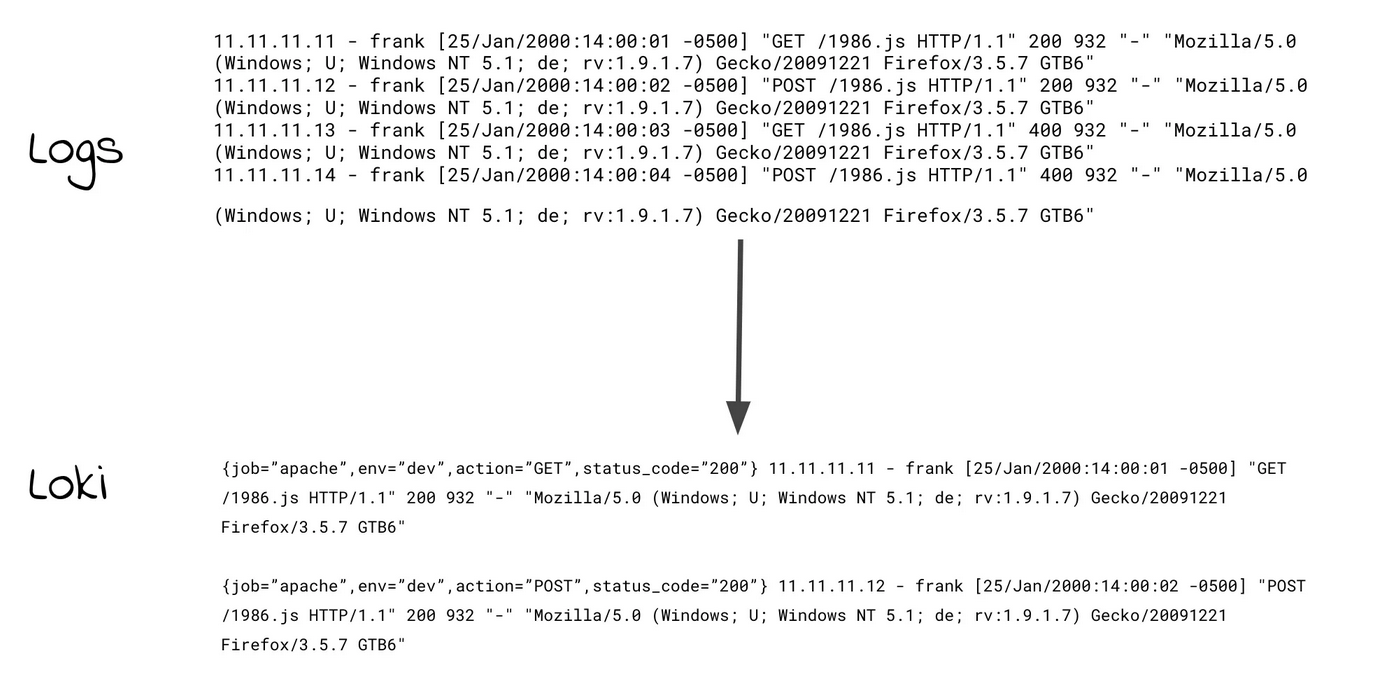
\includegraphics[width=1\textwidth]{figures/loki-indexing}}
    \captionsetup{justification=centering}
    \caption{Exemple del funcionament de la indexació dels paràmetres a \textit{Grafana Loki}. (\textbf{Font}: \url{https://medium.com/geekculture/pushing-logs-to-loki-without-using-promtail-fc31dfdde3c6})}\label{fig:loki-indexing}
\end{figure}

\noindent \\
Malauradament, errors durant l’etapa de configuració, concretament del paràmetre que defineix el temps màxim d'anterioritat per la cerca dels \textit{\gls{log}s}, ens van fer recular i considerar altres opcions.

\clearpage

\noindent
La següent opció és \textit{InfluxDb}.
Aquesta base de dades, també basada en series temporals, té característiques similars a l’anterior:

\begin{itemize}
    \item Base de dades de codi obert compatible per diferents plataformes.
    \item És una eina ben documentada~\cite{influxdb:documentation}.
    \item Té una gran quantitat d’usuaris actius.
    El repositori de codi~\cite{influxdb:code} és mantingut activament i de forma actual.
    \item Integració per defecte amb Grafana per poder visualitzar els \textit{logs}.
    \begin{itemize}
        \item Aquest és un dels punts que ens van fer considerar aquesta opció, ja que va ser recomanada pel mateix aplicatiu de Grafana.
    \end{itemize}
    \item Diverses llibreries~\cite{influxdb:libraries} ja implementades per enviar \textit{\gls{log}s} a la base de dades.
    \begin{itemize}
        \item En el nostre cas emprar \textit{influxdb-client}~\cite{influxdb:python} pel llenguatge \textit{Python}.
    \end{itemize}
    \item En aquest cas, però, la indexació és a partir dels tags.
    Utilitzarem aquest camp per afegir valors freqüents, que poden ser agrupats i fàcilment indexats.
\end{itemize}

\begin{figure}[htbp]
    \centerline{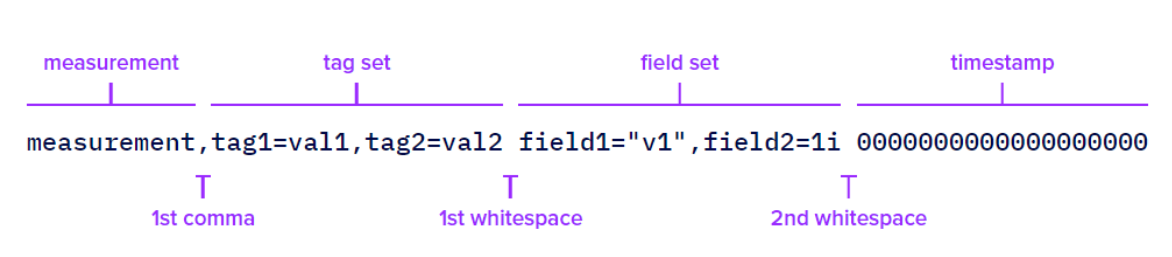
\includegraphics[width=1\textwidth]{figures/influxdb-indexing}}
    \captionsetup{justification=centering}
    \caption{Exemple del funcionament de la indexació dels paràmetres a \textit{InfluxDb}. (\textbf{Font:} \url{https://docs.influxdata.com/influxdb/v2/get-started/write/\#line-protocol-element-parsing})}\label{fig:influxdb-indexing}
\end{figure}

\clearpage

\subsection{Procés d'abocament dels \textit{\gls{log}s}}\label{subsec:log-push}

\noindent
El procés d’abocament dels \textit{\gls{log}s} consisteix a migrar tots els \textit{\gls{log}s} d’una estructura de fitxers, emmagatzemats en un directori, a un sistema gestor de bases de dades. \\

\noindent
Els \textit{\gls{log}s} es trobaven emmagatzemats a \texttt{/mnt/working/logsanon}, on hi havia un fitxer comprimit amb tots els registres per cada dia. \\

\noindent
Per tal de poder fragmentar la tasca, s’ha desenvolupat un petit \textit{script} que descomprimeixi aquests arxius, i el més important, seguint aquesta estructura de fitxers com a ubicació destí:

\begin{verbatim}
    2006
    |-- 01
    |   |-- 2006-01-01.log
    |   |-- ...
\end{verbatim}
\noindent
D’aquesta manera, podem realitzar l’abocament de manera esglaonada (any per any, mes a mes, etc.) i acotada.

\noindent \\
La base de dades escollida, com prèviament s’ha documentat~\ref{subsec:log-db-decision}, és \textbf{InfluxDb}.
Per tal de poder enviar les dades, hem fet ús de la llibreria oficial~\cite{influxdb:python} que ofereix la plataforma pel llenguatge Python.

\clearpage

\noindent
\textbf{Format de les dades} \\ \\
\textbf{InfluxDb} emmagatzema les dades utilitzant el que anomenen el ``Line protocol''.
Esquematitzant-ho, i amb el suport de la figura~\ref{fig:influxdb-indexing}, tractarem quatre paràmetres:

\begin{itemize}
    \item \texttt{measurement}: identificador principal de les dades.
    \item \texttt{tag set}: conjunt de parelles clau-valor \textbf{indexades}.
    Farem ús d'aquest camp per afegir valors freqüents, que poden ser agrupats i fàcilment indexats:
    \begin{itemize}
        \item \textbf{content}: format del contingut, pot ser:
        \begin{itemize}
            \item \texttt{ok}: el format del \textit{\gls{log}} és l'esperat.
            \item \texttt{diferent}: el format del \textit{\gls{log}} no és l'esperat però s'ha pogut tractar.
            \item \texttt{error}: error de processament.
        \end{itemize}
        Vegeu errors de processament~\ref{subsubsection:log-errors}.
        \item \textbf{method}: mètode \gls{HTTP} present al \textit{\gls{log}}.
        \item \textbf{status\_code}: codi d'estat de la resposta de la petició d'\gls{HTTP} .
        \item \textbf{type}: tipus de \textit{\gls{log}}, pot ser:
        \begin{itemize}
            \item \texttt{cerca}: cerca a la plataforma d'\gls{UPCommons}.
            \item \texttt{recurs}: accés a un recurs d'\gls{UPCommons}.
            \item \texttt{altres}: altres tipus de \textit{\gls{log}}.
        \end{itemize}
        Vegeu filtrage dels \textit{\gls{log}s}~\ref{subsec:log-filter}.
    \end{itemize}
    \item \texttt{field set}: conjunt de parelles clau-valor \textbf{no indexades}.
    Aquí hi emmagatzemarem valors únics, com són:
    \begin{itemize}
        \item \textbf{log}: registre complet d'\gls{UPCommons}.
        \item \textbf{recurs}: identificador \gls{handle}, en cas que es tracti d'un accés a un recurs.
    \end{itemize}
    \item \texttt{\gls{timestamp}}: marca temporal en nanosegons.
\end{itemize}

\clearpage

\noindent
\textbf{Optimitzacions} \\ \\

\noindent
La implementació del client d'InfluxDb ha estat optimitzada~\cite{influxdb:optimizations} de la següent manera:

\begin{itemize}
    \item \texttt{batching}: El mode d'escriptura emprat és el \textit{batching}.
    Consisteix a agrupar els elements (\textit{\gls{log}s}) en tandes, i després enviar una petició d'escriptura.
    A causa del volum de dades que tractem, evitem enviar una petició per cada \textit{log}, alleugerint la càrrega computacional.
    \begin{tcolorbox}[colback=red!5!white, colframe=red!75!black, title=Sobrecàrrega]
    En cas de disposar de la base de dades en algun servei de \textit{cloud}, aquest problema s'agreujaria, incrementant la latència.
    \end{tcolorbox}
    \item \texttt{flush\_interval}: La mida de les tandes (\textit{batches}) és de 500 elements.
    A part d’això, establim una marca temporal mínima en què s’envien les dades.
    És a dir, enviem una petició d’escriptura si es compleix alguna de les següents condicions:
    \begin{itemize}
        \item S’ha arribat a la mida del \textit{batch}: 500.
        \item Ha passat dos segons des de la darrera petició d’escriptura.
    \end{itemize}
    \item \texttt{tags}: El diccionari que conté les etiquetes amb informació rellevant del \textit{\gls{log}} s’ha ordenat alfabèticament a partir de les claus.
    \item \texttt{\gls{timestamp}}: Enviem el \textit{\gls{log}} amb la marca temporal amb precisió de l’orde dels nanosegons, format que utilitza \textbf{InfluxDb}.
    \item \texttt{\gls{gzip}}: comprimint les dades podem accelerar el procés d’escriptura fins a cinc vegades, tal com indica la guia d'optimització d'InfluxDb~\cite{influxdb:optimizations}
\end{itemize}

\clearpage

\noindent
\textbf{Estadístiques} \\ \\

\noindent
El resultat de l’abocament conclou amb la taula~\ref{tab:logs-table} on es mostren alguns números interessants.
Per cada columna, tenim els següents camps:

\begin{itemize}
    \item Nombre total de \textit{\gls{log}s}:
    \begin{itemize}
        \item Nombre total de \textit{logs} processats.
    \end{itemize}
    \item Accés a recursos d'\gls{UPCommons}:
    \begin{itemize}
        \item Aquells registres que accedeixen a recursos d’UPCommons. 
        Es té en compte els següents dos casos:
        \begin{itemize}
            \item Contenen l’identificador \gls{handle} present.
            \item Content el \gls{bitstream} \gls{UUID} present.
        \end{itemize}
    \end{itemize}
    \item Cerques a \gls{UPCommons}:
    \begin{itemize}
        \item Aquells registres que cerquen a través de la plataforma d’\gls{UPCommons}.
    \end{itemize}
    \item Accés a recursos web descartats:
    \begin{itemize}
        \item Registres que corresponen a accessos a recursos web del servidor i que no ofereixen cap més informació.
    \end{itemize}
    \item Altres tipus de \textit{logs}:
    \begin{itemize}
        \item Aquells registres que no concorden amb cap característica prèviament mencionada.
        No són ni recursos \gls{UPCommons}, ni cerques, ni tampoc recursos web.
    \end{itemize}
    \item Errors de processament:
    \begin{itemize}
        \item Aquests casos corresponen a malformacions greus del \textit{\gls{log}} que tenen com a conseqüència no poder ser analitzats adequadament.
    \end{itemize}
    \item Duració de l’abocament:
    \begin{itemize}
        \item Temps necessitat per dur l’abocament.
        Comptabilitzem des que s’insereix el primer registre d’aquell rang fins a l’últim.
    \end{itemize}
\end{itemize}